\minitoc

\section{Motivation}
\label{S_motivation_intro}
The Internet of Things (IoT) is a unique paradigm, with an estimated 15.1 billion active devices in 2023 (cf. Figure \ref{F_devices_forecast}) connecting and exchanging data through different communication networks~\cite{StatistaIoT2023}. With a forecast number of active devices reaching 29.4 billion by 2030~\cite{StatistaIoT2023}, the requirements regarding performance, security and privacy in the Internet of Things will be increasingly pressuring. Numerous domains of activities are to be impacted, including, but not limited to, healthcare, industries, cities, logistics, agriculture or construction (cf. Figure \ref{F_devices_forecast} categories).

\begin{figure}[t]
\centering
 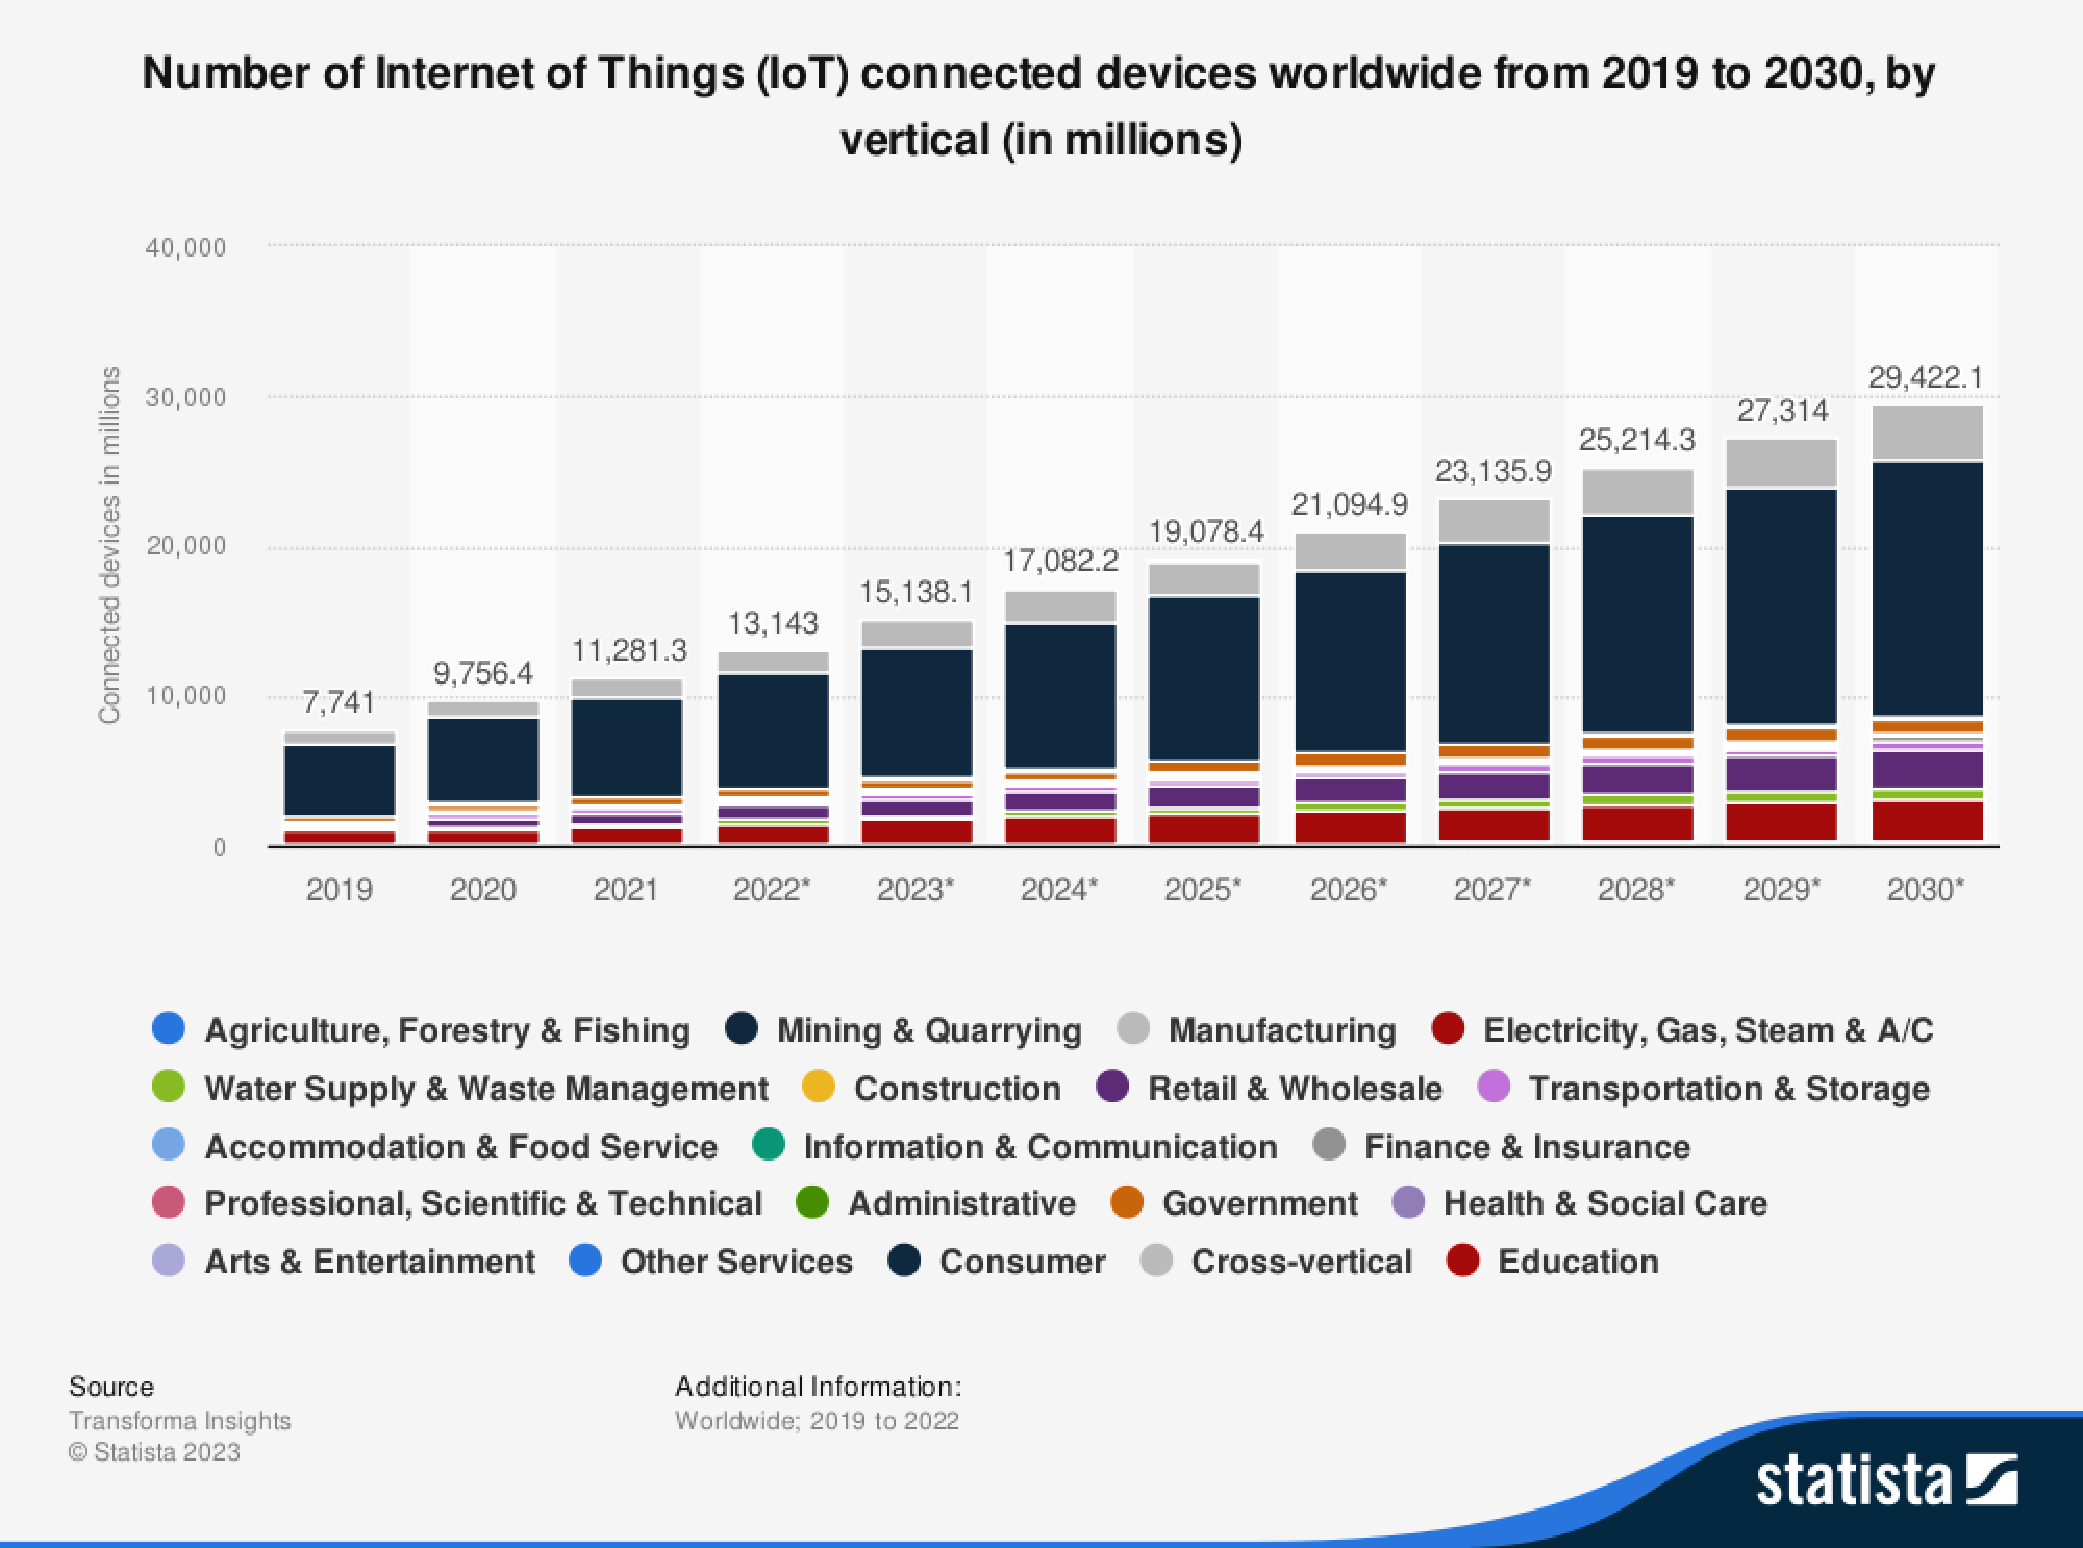
\includegraphics[scale=0.4]{Images/devices_forecast.pdf}
\caption[Number of Internet of Things (IoT) connected devices worldwide from 2019 to 2030, by vertical]{Number of Internet of Things (IoT) connected devices worldwide from 2019 to 2030, by vertical. The single largest use case in terms of the number of Internet of Things (IoT) connected devices is consumer internet and media devices, accounting for a third of all devices worldwide in 2030. The other two largest use cases are smart grid (e.g. smart meters) and connected vehicles - Statista \cite{StatistaIoT2023}}
\label{F_devices_forecast}
\end{figure} 
\textbf{Security and privacy risks.}
The Internet of Things (IoT) is bringing new ways to collect data, analyze them and take decisions
for developing applications that answer or even anticipate the users’ needs. The unprecedented nature of the IoT has consequences on the data generated, which are \emph{fine-grained} and in \emph{quantity}.\sul{ The collected data enables the monitoring of users' actions and locations while users are often unaware of the data collection}. For these reasons, the data are particularly
privacy-sensitive, requiring efficient privacy-preserving mechanisms. Moreover, the IoT has unique
characteristics due to the extreme heterogeneity and large quantity of objects it can interconnect, as
well as the spontaneous nature of their interactions, making it a distributed system of unprecedented
scale. It results in several security complications, as some IoT devices, e.g., sensors, may not have the computation power or storage needed to implement 
cryptographic primitives. Additionally, IoT devices may have security vulnerabilities in their firmware, software, or hardware components. These vulnerabilities can be exploited to gain control over devices, disrupt their functionality, or launch attacks on other devices or networks \cite{Omolara2022}.

\textbf{Regulation.} Furthermore, the EU General Data Protection Regulation (GDPR) \cite{EUdataregulations2018} introduces several legal obligations, among which \emph{privacy-by-default}, \emph{consent management} and \emph{accountability}. Indeed, companies - outside of the legitimate interest - have to explicitly ask the user,
as a data owner, for clear, positive and explicit consent before any data collection. Whatever the
interests at stake, a company has to prove at any time that data processing is always performed
legitimately, either according to the user’s consent or for a legitimate purpose.

\textbf{Requirements for a secure Internet of Things.}
\cul{As a consequence of the security and privacy risks peculiar to the Internet of Things, the requirements for a secure and privacy-preserving Internet of Things are the following. First, the solution must consider} \emph{constrained devices},
\cul{and ensure the security and privacy threat mitigations are not disconnected 
from IoT's actual capacities. For example, cryptography-based solutions are often inapplicable to Internet of Things devices. Second, as data are privacy-sensitive, it is compulsory for user's privacy to enforce} \emph{access control} on their data and to \emph{monitor the usage of their data}. \cul{Third, for performance, security and privacy purposes, decentralization is an important aspect in the Internet of Things. Centralized entities such as cloud servers may snoop on users' data}~\cite{Qin2020} and can be vulnerable to accidental disclosures or external attacks~\cite{Qin2020}. Availability can be a matter of concern too, as physical infrastructure can be damaged, e.g. because of a fire or a natural disaster~\cite{Ayoub2021}. Furthermore, centralization hinders performance, specifically by increasing the deployment and maintenance cost~\cite{Salimitari2020}, which in turn hinders scalability.

\textbf{Leveraging distributed ledgers for the Internet of Things.} \cul{Distributed ledger technologies (DLTs), due to inherent properties, are a promising solution to address the Internet of Things requirements for security. DLTs indeed provide a certain degree of \emph{decentralization} and are \emph{tamper-proof} which is useful for a wide range of security applications ranging from trust management} \cite{Liu2023} \cul{to anonymous and secure transactions} \cite{Bothra2023}. \cul{DLTs can also be used to provide access control in an automated and transparent fashion using \emph{smart contracts}} \cite{Bao2023}. \cul{However, distributed ledger technologies are not always designed for the Internet of Things requirements. Performance, security and privacy requirements call for well-tailored distributed ledgers, that provide anonymous, efficient and cheap transactions for IoT-constrained devices.}

\section{Problem statement}
\label{S_problem_statement}
\sul{In this part, several challenges related to the Internet of Things are highlighted
and are used to identify \emph{research objectives}. These objectives will provide the connecting thread throughout this document.}
\paragraph{Micro-transactions.} In the Internet of Things, data collection often serves business purposes and requires financial transactions afterward to buy and sell the data. Data trading is based on \emph{micro-transactions}, which should be processed with the minimum possible fee as regards the data value. Additionally, several Internet of Things real-life scenarios without data trading require micro-transactions. Such use cases include \emph{parking meters} in smart cities, where the drivers would be charged automatically for the amount of time they park their vehicles. In \emph{Industrial Internet of Things} (IIoT), IoT devices could monitor machinery and equipment and automatically order replacement parts for improved maintenance. The manufacturer could be charged a small fee for the replacement parts, with the payment occurring automatically via micro-transactions.

Overall, micro-transactions can provide new revenue streams for businesses by enabling them to monetize data generated by IoT devices and 
increase the efficiency of business operations by enabling automated payments.
However, it is important to ensure that privacy and security are maintained to protect sensitive data due to the Internet of Things context and financial transactions involved.
The latter issues as well as the need for efficient, micro-transactions in the IoT leads to the first research objective of this thesis:
\begin{mdframed}[ skipabove=20pt, skipbelow=20pt, innertopmargin=12pt, innerbottommargin=12pt] 
\phantomsection    
\begin{center}
     \emph{Objective 1: Achieve privacy-preserving zero-fee transactions for the Internet of Things} 
     \label{obj:1}
\end{center}
\end{mdframed}

%\paragraph{Distributed ledgers and privacy-enhancing technologies.} To make transactions, blockchains or distributed ledgers in general are technologies of interest in IoT settings due to their inherent distribution.
%Besides, due to its unique properties, the use of distributed ledger technologies with privacy-enhancing technologies, including usage control, has been widely discussed in the literature \cite{Cha2019}. There are three main categories for the use of distributed ledgers in PETs: access control, auditing and data storage \cite{Cha2019}.  
%Notably, distributed ledgers are used for their smart contracts to define and enforce access policies of the data \cite{Khan2020, Zhaofeng2021, Bao2023, Rifi2017}. As regards usage control, several works have been conducted in private blockchain settings \cite{Khan2020, Zhaofeng2021, Shi2021}. While private blockchains benefit from low latency, they lack some beneficial features of public distributed ledgers such as total distribution with highly secure and immutable data storage. Besides, the network overhead increases rapidly with the number of nodes in the PBFT consensus protocol, commonly used by private blockchains.  \cite{Salimitari2020}. Distributed ledgers often have performance constraints that do not meet IoT requirements, such as the number of transactions per second \cite{Salimitari2020}.

\paragraph{Distributed ledgers and usage control.} To process transactions, blockchains or distributed ledgers in general are technologies of interest in IoT settings due to their inherent distribution.
Besides, due to its unique properties, the use of blockchains jointly with usage control has been widely discussed in the literature. \sul{Usage control can be considered as an extension of access control, which continuously monitors data once access has been granted. It grants or denies access based on \emph{authorizations}, \emph{obligations}, which have to be fulfilled to be granted access, and finally on \emph{conditions}
related to the system state. As a consequence, usage control is beneficial to users' privacy as they can decide who may access their data and how the data are used.}

Several works combining usage control and blockchains have been conducted in private blockchain settings \cite{Khan2020, Shi2021, Zhaofeng2021, Zhang2022}. While private blockchains benefit from low latency, they lack some beneficial features of public distributed ledgers such as total distribution with highly secure and immutable data storage. Besides, the network overhead increases rapidly with the number of nodes in the PBFT consensus protocol, commonly used by private blockchains.  \cite{Salimitari2020}. Distributed ledgers often have performance constraints that do not meet IoT requirements, such as the number of transactions per second \cite{Salimitari2020} \sul{which is around 6 transactions per second (TPS) for the Bitcoin blockchain excluding use cases with numerous simultaneous transactions. The size of the transaction ledger can be a hurdle to IoT adoption as well. The Bitcoin blockchain has grown to 475 GB as of June 8, 2023, which is impossible to store on lightweight devices} \cite{StatistaBTC2023}

 Even though the literature proposed integration schemes for usage control in distributed ledgers \cite{Khan2020, Shi2021}, the general principles of integration are not properly identified. In particular, solving the potential bottleneck issues, as well as the identification of criteria for integration, are not well addressed by the current research.
Considering these current limitations, this thesis identifies the following research objectives: 
\phantomsection 
\begin{mdframed}[ skipabove=20pt, skipbelow=20pt, innertopmargin=12pt, innerbottommargin=12pt] 
\begin{center}
     \emph{Objective 2: Identify the distributed ledgers appropriate for the Internet of Things} 
    \newline


   \emph{Objective 3: Design a method to integrate usage control in distributed ledger technologies efficiently}
   \label{obj:23}
\end{center}
\end{mdframed}
\paragraph{Data usage control modeling in distributed systems.}
A formal model of data usage control can help ensure that the system's security and privacy goals are achieved by providing a clear specification of the access control policies, the resources to be protected, and the roles and responsibilities of the participants in the system. 
While this modeling has been repeatedly discussed in the state of the art in centralized settings \cite{Pretschner2011, Kelbert2013, Kelbert2014, Fromm2020}, it is still incomplete in distributed systems \cite{Gil2023}, considering only the distribution of the usage control system (UCS) components, but not of the other system users, such as the policy makers and the data readers \cite{Kelbert2015, Kelbert2018}.
In the Internet of Things, due to performance, security and privacy concerns, distributed systems are widely used, requiring 
an appropriate model to describe information flows and data policies. This leads to the introduction of the fourth research objective:
\phantomsection 
\begin{mdframed}[ skipabove=20pt, skipbelow=20pt, innertopmargin=12pt, innerbottommargin=12pt] 
\begin{center}
     \emph{Objective 4: \cul{Identify concepts relevant to the Internet of Things and missing from the current usage control formalism in distributed systems}} 
     \label{obj:4}
\end{center}
\end{mdframed}

\textbf{Validation of the proposed solutions.} \cul{As part of the previous research objectives (Objectives 1 to 4), several solutions will be proposed in this thesis work to address specific issues in the Internet of Things. As regards the performance, security and privacy constraints of the IoT, it is necessary that: 1) the security and the privacy of these solutions are assessed; 2) the solutions are tested using \emph{proof of concepts} to ensure their feasibility, in particular, as regards performance.} \cul{These requirements lead to 
the last set of research objectives}:

\phantomsection 
\begin{mdframed}[ skipabove=20pt, skipbelow=20pt, innertopmargin=12pt, innerbottommargin=12pt] 
\label{obj:5_6}    
    \begin{center}
         \emph{Objective 5: Analyze the security and privacy of the proposed methods with security and/or privacy threat assessment} 
        \newline
    
    
       \emph{Objective 6: Validate the feasibility of the proposed methods with 
       a proof of concept}
       \newline 
       
       %\emph{Objective 7: Validate the modeling of data usage control in distributed systems using model checking}
       \label{obj:56}
    \end{center}
    \end{mdframed}

\section{Assumptions}
\label{S_assumptions}

The Internet of Things encompasses a wide range of use cases with different requirements and specific research questions. As a consequence, this section explains the context considered in this thesis. Several definitions are first provided to clarify some notions such as the Internet of Things. \rul{The initial assumptions at the start of the Ph.D. are then provided, to highlight the results of the analysis of the state of the art.} The precise context considered is finally given to define the scope of the conducted research.

\paragraph{Definitions.} The \emph{Internet of Things}, i.e., IoT for short, has been first used in 1999 by MIT's Kevin Ashton when he promoted the RFID technology \cite{Zhang2020}. The Internet of Things has since disrupted the classic Internet by introducing devices embedded in everyday objects, sending and receiving data by themselves. However, the actual definition of the Internet of Things is loose and is often referred to using other words such as \emph{smart home} outside academia and industry \cite{Berte2018}. The National Institute of Standards and Technology (NIST) agrees with the lack of a universal definition of the Internet of Things but proposes the two following \emph{fundamental concepts} of the IoT \cite{NISTIR8200}:
\begin{center}
\begin{mdframed}[ skipabove=20pt, skipbelow=20pt, innertopmargin=12pt, innerbottommargin=12pt] 
\begin{itemize}
    
    \item[(1)] \emph{IoT components are connected by a network providing the potential for a many-to-many
relationship between components (the network capability may or may not be
Transmission Control Protocol/Internet Protocol (TCP/IP) based)};
    \item[(2)] \emph{Some IoT components have sensors and actuators that allow the components to observe
(collect data about) and affect the physical world.}
\end{itemize}
\end{mdframed} 
\end{center}

These two concepts are of interest as they reflect the \emph{high number of devices}, the \emph{heterogeneity} both in terms of protocols and devices, and the link between the IoT devices and the physical world.

Similarly, \emph{privacy} is repeatedly mentioned in this thesis but is not an easy concept to define. It is recurrently discussed in the literature \cite{Moore2008,  Alibeigi2019, Tang2021, Elmimouni2023} and derived to more precise concepts, such as \emph{usable privacy} \cite{Malkin2023} which refers to the implementation of user-friendly privacy-preserving mechanisms. For privacy, the two following definitions are proposed, first to emphasize the interdisciplinary aspect of privacy, then a definition more related to data and computer science, also called \emph{information privacy}:

\begin{center}
\begin{mdframed}[ skipabove=20pt, skipbelow=20pt, innertopmargin=12pt, innerbottommargin=12pt] 
\begin{itemize}
    \item[(1)] \emph{Broadly speaking, privacy is "the right to be let alone" \cite{Warren1890}, or freedom from interference or intrusion}; 
    \item[(2)] \sul{\emph{Privacy is the claim of individuals, groups, or institutions to determine for themselves when, how, and to
    what extent information about them is communicated to others}} \cite{Westin1968}.
\end{itemize} 
\end{mdframed}
\end{center}

\cul{To further clarify the notion of privacy, we list the privacy properties of interest for this thesis work. 
Users tend to provide excessive information to
service providers and to lose control of their personal information. Therefore, the \emph{content awareness (1)} property is proposed} \cite{Wuyts2015}
 \cul{to make sure that users are aware of their personal data
and that only the minimum necessary information should be
shared and used for data processing.
The more personally identifiable information a data subject discloses, the higher the risk is for a privacy violation. To
ensure content awareness, several technical enforcement tools have been developed such as the personal information feedback tools} \cite{Patil2009} \cul{to help users gain privacy awareness and self-determine which personal data to disclose.}

\cul{Unlike the user-centric content awareness property, the \emph{policy and consent compliance} property (2)} \cite{Wuyts2015} \cul{requires
the whole system, e.g., including data flows, data stores, and
processes, as a data controller to inform the data subjects
about the system's privacy policy, or allow the data subjects
to specify consent in compliance with the legislation. These two properties are often referred to as 
\emph{soft privacy}} \cite{Wuyts2015}. \cul{\emph{Hard privacy} focuses on 
providing as little data as possible to reduce the need to trust other entities, which is referred to as \emph{data minimization}. On the contrary, soft privacy is based on the assumption
that data subjects have already no control over their personal data and must
have confidence in data controllers. The
data protection purpose of soft privacy is therefore to provide data security and process data with specific purpose and consent,
using policies, access control, and audit}.  

\paragraph{\rul{Initial assumptions.}} \rul{To provide a better understanding of the contributions of this thesis work, we describe here the assumptions at the beginning of the Ph.D. work. First, the initial research questions were the following:}

\begin{enumerate}
    \item Which privacy-enhancing technologies are suitable for the Internet of Things? 
    \item How to enable usage control in distributed IoT platforms in an efficient way?
\end{enumerate}

\rul{While doing the state of the art, which is summarized in the dedicated Chapter} \ref{C_state_of_the_art}, \rul{it appeared that instead of identifying PETs for the Internet of Things, it was more relevant to address performance and security requirements, then to implement privacy-enhancing technologies on the chosen technologies. Indeed, privacy-enhancing technologies can add overhead to the already performance-demanding Internet of Things. Addressing privacy before the performance aspects would be poorly satisfying, due to the impossibility to implement the proposed privacy-preserving solutions in practice. As a result of the analysis of the state of the art, blockchains, first of all, then distributed ledgers appeared as a technology of interest for performance and security. Indeed, blockchains are decentralized by nature and address numerous issues existing in centralized networks, including availability with the removal of a single point of failure, but also performance with better scalability, reduced maintenance costs and reduced update costs} \cite{Salimitari2020}.

% \rul{No hypothesis on the most suitable blockchain technology was formulated at the beginning of the Ph.D., nor were the scenarios used in Chapter} \ref{C_solving_trilemma} \rul{and Chapter} \ref{C_formalism} \rul{defined}.

\paragraph{Context.} In this thesis, only \emph{large-scale IoT deployments} are considered, as use cases involving a moderate amount of devices are already well addressed by the state of the art. Large-scale IoT deployments have specific issues regarding scalability, heterogeneity and performance constraints on devices that require dedicated, well-tailored solutions. For instance, private blockchains, often considered as an IoT-friendly technology \cite{Asheralieva2021}, are actually not well-suited for large-scale deployments of devices. 

Second, the scenarios considered will require \emph{payments}, as IoT devices can be used in real-life to generate and sell data or buy actual goods, e.g., vending machines. Finally, the Internet of Things features a high diversity of devices. This \emph{heterogeneity} of devices is considered in this thesis, which implies that constrained devices, e.g., in terms of computing power, memory, energy storage..., are involved in the network. This last assumption markedly restricts the use of several security and privacy tools, such as encryption. \rul{While this thesis work considers the heterogeneity of devices, it does not address every Internet of Things use-cases. For instance, the Industrial Internet of Things devices may operate in a closed environment preventing them from selling the data to outside agents. Besides, actuators do not have an obvious incentive to trade their data or even generate data in the first place.}

\rul{For a better understanding, we provide scenarios where data trading could be relevant:}
\begin{itemize}
    \item \emph{agriculture and precision farming}: farmers can collect data from IoT sensors installed in fields to monitor soil moisture, temperature, humidity, and crop growth. This data could be aggregated and sold to agricultural technology companies or research institutions to improve crop yield and develop new farming techniques;
    \item \emph{smart city infrastructure}: municipalities can gather data from IoT devices deployed throughout the city to monitor traffic patterns, air quality, waste management, and energy consumption. This data could be valuable for urban planning, transportation optimization, and environmental monitoring, and could be sold to city planners or companies working on smart city solutions;
    \item \emph{smart home}: manufacturers of smart home devices, such as thermostats, security cameras, and smart appliances, might offer users the option to sell usage data. This data can provide insights into user preferences and usage patterns, helping manufacturers refine their products;
\end{itemize}
\rul{Conversely, the following families of scenarios are out of the scope of this thesis:}
\begin{itemize}
    \item \emph{closed environments}, such as \emph{manufacturing} where there is a lack of incentive to buy or sell actuator data; 
    \item \emph{specific legislations}, such as medical data legislations in the \emph{e-health} sector. Several legislations have strict rules as regards the selling of medical data, for privacy reasons. Data trading may be impossible in some use cases, or without the clear and explicit consent of the users.
\end{itemize} 

\section{Contributions}

This thesis addresses the defined research objectives with the following contributions:

\begin{itemize}
    \item the design of a framework to address the requirements of privacy, security and performance of the Internet of
Things (Chapter \ref{C_solving_trilemma}). The basis of the framework is the IOTA technology, a distributed ledger relying on a directed acyclic graph to create zero-fee transactions, instead of a blockchain (\hyperref[obj:1]{\emph{Objective 1}} and \hyperref[obj:23]{\emph{Objective 2}}). A security and privacy threat assessment is conducted on the proposed solution using an illustrative scenario of a car sharing system (\hyperref[obj:56]{\emph{Objective 5}} and \hyperref[obj:56]{\emph{Objective 6}});
\item an integration method of usage control with distributed ledgers (Chapter \ref{C_integration}). Suitable DLTs are determined according to specified parameters, and a proof of concept is proposed for performance evaluation (\hyperref[obj:23]{\emph{Objective 3}} and \hyperref[obj:56]{\emph{Objective 6}}). A privacy threat assessment using LINDDUN is also conducted (\hyperref[obj:56]{\emph{Objective 5}});
\item an extension of a decentralized model for usage and
information flow control in distributed systems, introducing a policy jointly defined over collective personal data and \cul{ considering the
availability of the different individual parts of the distributed system} (\hyperref[obj:4]{\emph{Objective 4}});
\end{itemize}

\textbf{Framework for performance, privacy and security in the Internet of Things. } 
This first contribution (\emph{Contribution 1}) proposes a newly designed framework to address the requirements of privacy, security and
performance of the Internet of Things. In this contribution, we first identify IOTA as the basis of the framework and demonstrate its relevance. IOTA indeed unlocks distributed ledger performance by increasing throughput as more users join the
network thus making the network scalable. Additionally, IOTA does not rely on miners to add transactions to the ledger, enabling zero-fee transactions. Not designed for privacy protection, IOTA is complemented in the framework by privacy-preserving mechanisms: merge avoidance
and decentralized mixing. Finally, usage control mechanisms are introduced so that users can monitor the use and dissemination of their data.

\textbf{Integration of usage control with distributed ledgers.} This contribution  (\emph{Contribution 2}) proposes to integrate usage control with distributed ledgers based on directed
acyclic graphs (DAG). The benefits of integration are: 1) the components of the usage control system contribute
to the network security, as a node; 2) the usage control
system processes the transaction data without intermediaries,
which is faster and more reliable. An analysis of
distributed ledgers is provided based on their features, to determine which
ledgers are suitable for the proposed integration. An implementation of usage control integration is proposed on IOTA. Performance tests are conducted on this implementation, showing approximately a 90\% decrease
in the time needed to push transactions and make an access decision when the UCS is integrated.

\textbf{Data usage control modeling in distributed systems.} The last contribution (\emph{Contribution 3}) of this thesis work is the proposition of an extended usage control model \sul{going beyond the state of the art} that integrates decentralized information flow control (DIFC). DIFC enables users to decide collectively which policy to apply to their common data, \sul{further distributing the network by decentralizing the policy definition to the users}.
Architectural aspects and formal definitions to enable decentralized policies for shared data are proposed as a novelty, resulting from the DIFC integration.
Unreliable and intermittent distributed systems are also considered, as a distinctive characteristic in some Internet of Things use cases, e.g., low-energy devices. 

\section{Acknowledgments}

This thesis work and the associated Ph.D. have been funded by the
Futures \& Ruptures program of Foundation Mines-Télécom. It is also partially supported by the Institut Mines-Télécom VP-IP Chair on Values and Policies of Personal Information (\url{https://cvpip.wp.imt.fr}) and by the 3rd Programme d’Investissements d’Avenir [ANR-18-EUR-0006-02]
within the framework of Energy4Climate Interdisciplinary Center (E4C) of IP Paris and Ecole des Ponts ParisTech (\url{https://www.e4c.ip-paris.fr/}). 

\section{Thesis outline}

This document is structured as follows. Chapter \ref{C_state_of_the_art} provides the necessary background on usage control and distributed ledgers, then the state of the art and \cul{its current limitations in addressing the different objectives of the problem statement} (cf. Section \ref{S_problem_statement}). Chapter \ref{C_solving_trilemma} details the design of a framework (\emph{Contribution 1}) to simultaneously address performance, security and privacy requirements in the Internet of Things and enable micro-transactions (\hyperref[obj:1]{\emph{Objective 1}}). \sul{The framework is based on the IOTA distributed ledger, and its security and privacy are evaluated on a car-sharing use case}. Chapter \ref{C_integration} details the integration of usage control with distributed ledgers (\emph{Contribution 2}) to further improve the performances of both the distributed ledger and usage control system. Chapter \ref{C_formalism} addresses the issues in defining a formalism for usage control in distributed systems and justifies the use of decentralized information flow control to complete the state-of-the-art formalism (\emph{Contribution 3}). The final Chapter \ref{C_conclusion} concludes this thesis with a summary of the thesis, the future works and the limitations considering both the research objectives and the scope of this research work.
A glossary (Appendix \ref{A_glossary}) provides definitions and explanations for some notions 
for better understanding.
The complementary appendices (Appendix \ref{A_cryptocurrencies}, Appendix \ref{A_usage_control}) provide additional general information on the different technologies 
addressed in this thesis.  